\documentclass[12pt]{article}
\usepackage[english]{babel}
\usepackage[utf8x]{inputenc}
\usepackage[T1]{fontenc}
\usepackage{scribe}
\usepackage{listings}
\usepackage{graphics, graphicx}
\usepackage{enumitem}
\usepackage{tcolorbox}
\usepackage{adjustbox}
\usepackage{float}
\usepackage{mathtools}
\usepackage{tikz}
\usepackage{wrapfig}
\usepackage{tcolorbox}
\usepackage{amsthm}

\makeatletter
\newcommand*{\rom}[1]{\expandafter\@slowromancap\romannumeral #1@}
\makeatother
\graphicspath{ {./images/} }

% Default fixed font does not support bold face
\DeclareFixedFont{\ttb}{T1}{txtt}{bx}{n}{12} % for bold
\DeclareFixedFont{\ttm}{T1}{txtt}{m}{n}{12}  % for normal

% Custom colors
\usepackage{color}
\definecolor{deepblue}{rgb}{0,0,0.5}
\definecolor{deepred}{rgb}{0.6,0,0}
\definecolor{deepgreen}{rgb}{0,0.5,0}

\usepackage{listings}

% Python style for highlighting
\newcommand\pythonstyle{\lstset{
    language=Python,
    basicstyle=\ttm,
    otherkeywords={self},             % Add keywords here
    keywordstyle=\ttb\color{deepblue},
    emph={MyClass,__init__},          % Custom highlighting
    emphstyle=\ttb\color{deepred},    % Custom highlighting style
    stringstyle=\color{deepgreen},
    frame=tb,                         % Any extra options here
    showstringspaces=false            % 
}}


% Python environment
\lstnewenvironment{python}[1][]
{
\pythonstyle
\lstset{#1}
}
{}

% Python for external files
\newcommand\pythonexternal[2][]{{
\pythonstyle
\lstinputlisting[#1]{#2}}}

% Python for inline
\newcommand\pythoninline[1]{{\pythonstyle\lstinline!#1!}}
\definecolor{commentgreen}{RGB}{128,128,128}
\definecolor{eminence}{RGB}{2,112,10}
\definecolor{weborange}{RGB}{255,165,0}
\definecolor{frenchplum}{RGB}{129,20,83}
\lstset {
	language=java,
	frame=single,
	tabsize=4,
	showstringspaces=false,
	numbers=left,
	commentstyle=\color{commentgreen},
	keywordstyle=\color{eminence}\bfseries,
	stringstyle=\color{red},
	basicstyle=\small\ttfamily, % basic font setting
	emph={int,char,double,float,unsigned,void,bool},
	emphstyle=\color{blue}\bfseries,
	escapechar=\&,
	classoffset=1,
	morekeywords={>,<,.,;,,,-,!,=,~},
	classoffset=0,
	xleftmargin=.05\textwidth, 
	xrightmargin=.02\textwidth
}
\newcommand{\verteq}{\rotatebox{90}{$\,=$}}
\newcommand{\equalto}[2]{\underset{\scriptstyle\overset{\mkern4mu\verteq}{#2}}{#1}}
\newcommand{\norm}[1]{\left\lVert#1\right\rVert}


\CourseName{Comtemporary Algorithms T.II/2019-20}
\Scribe{Pitipat C. \& Nuttapat K.}
\Lecturer{Dr. Kanat T.}
\LectureNumber{12}
\LectureDate{12 February 2020}
\LectureTitle{Linear Algebra}

\lstset{style=mystyle}

\newlist{steps}{enumerate}{1}
\setlist[steps, 1]{label = Step \arabic*:}

\begin{document}
\MakeScribeTop

%#############################################################
%#############################################################
%#############################################################
%#############################################################

\section{Notations}
\begin{description}
    \item[Vector]
        \begin{align*}
            \vec{v} &= (v_1, v2, \dots, v_d) \in \mathbb{R}^d\\
                    &= [v_1, v_2, \dots, v_d]^T \\
                    &= \begin{bmatrix} v_1 \\ v_2 \\ \vdots \\ v_d \end{bmatrix}  
        \end{align*}
    \item[Matrix]
        \begin{align*}
            && A &= \begin{bmatrix} 
                    a_{11} & a_{12} & \dots & a_{1d} \\
                    a_{11} & a_{12} & \dots & a_{1d} \\
                    \vdots &        & \ddots & \\
                    a_{n1} & \dots  & \dots      & a_{nd} 
                    \end{bmatrix} \in \mathbb{R}^{nxd} && \\
           &&   &= [\vec{a_1}, \vec{a_2}, \dots, \vec{a_d}] && \text{(MathLab Syntax)}\\  
           &&   &= \begin{bmatrix}- \vec{a_1}- \\ -\vec{a_2}- \\ -\vdots -\\ -\vec{a_d}- \end{bmatrix} && 
        \end{align*}
    \item[Linear Equations]
    \begin{align*}
        \equalto{\begin{array}{r@{\ }c@{\ }l}
                ax_1 & +bx_2 & +cx_3 = d \\
                ex_1 & +fx_2 & +gx_3 = h
            \end{array}
        }{\underbrace{\left[\begin{matrix}a&b&c\\e&f&g\end{matrix}\right]\begin{bmatrix} x_1 \\ x_2 \\ x_3 \end{bmatrix} = \begin{bmatrix} d \\ h  \end{bmatrix}}_{Ax=b}}
    \end{align*}
            
\end{description}

\section{Vector-Vector Products}
Let
\begin{align*}
    && \vec{x} = \begin{bmatrix} x_1 \\ x_2 \\ \vdots \\ x_d \end{bmatrix}, \vec{y} &= \begin{bmatrix} y_1 \\ y_2 \\ \vdots \\ y_d \end{bmatrix},
    \vec{z} = \begin{bmatrix} z_1 \\ z_2 \\ \vdots \\ z_d \end{bmatrix}&& \vec{x},\vec{y}, \vec{z} \in \mathbb{R}^d \\
    && \vec{v} &= \begin{bmatrix} v_1 \\ v_2 \\ \vdots \\ v_n \end{bmatrix}&& \vec{v} \in \mathbb{R}^n
\end{align*}

\subsection{Inner Product (Dot Product)}
    $$\vec{x} \cdot \vec{y} = \vec{x}^T\vec{y} = \langle \vec{x},\vec{y} \rangle = \sum_{i=1}^{d}x_iy_i$$
Dot product is \textbf{linear}.
\begin{align}
    \langle \alpha \vec{x},\vec{y} \rangle &= \alpha \langle \vec{x},\vec{y} \rangle \\ 
    \langle \vec{x},\vec{y}+\vec{z} \rangle &=  \langle \vec{x},\vec{y} \rangle + \langle \vec{x},\vec{z} \rangle
\end{align}
\begin{center}
    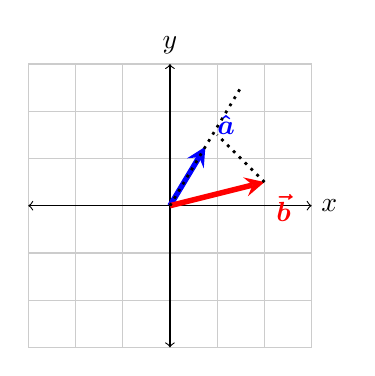
\begin{tikzpicture}[scale=0.6]
  \draw[thin,gray!40] (-3,-3) grid (3,3);
  \draw[<->] (-3,0)--(3,0) node[right]{$x$};
  \draw[<->] (0,-3)--(0,3) node[above]{$y$};
  \draw[line width=2pt,blue,-stealth](0,0)--(0.75,1.25) node[anchor=south west]{$\boldsymbol{\hat{a}}$};
  \draw[line width=2pt,red,-stealth](0,0)--(2,0.5) node[anchor=north west]{$\boldsymbol{\vec{b}}$};
  \draw[line width=1pt,dotted,black](0,0)--(1.5,2.5) node[]{};
  \draw[line width=1pt,dotted,black](2,0.5)--(1, 1.5) node[]{};
\end{tikzpicture}
\end{center}

\begin{align*}
    \langle \vec{a},\vec{b} \rangle &= \text{length of the projection of $\vec{b}$ onto $\vec{a}$} \\
    \langle \vec{a},\vec{b} \rangle &= \norm{\vec{a}} \norm{\vec{b}} cos \theta
\end{align*}

\subsection{Outer Product}
$$\vec{v} \cdot \vec{y}^T = \begin{bmatrix} v_1 \\ v_2 \\ \vdots \\ v_n \end{bmatrix}\begin{bmatrix}y_1&y_2&\dots&y_d\end{bmatrix} = \begin{bmatrix} d \\ h  \end{bmatrix} = \begin{bmatrix} 
                    v_1y_1 & v_1y_2 & \dots & v_1y_d \\
                    v_2y_1 & v_2y_2 & \dots & v_2y_d \\
                    \vdots &        & \ddots & \\
                    v_ny_1 & \dots  & \dots      & v_ny_d 
                    \end{bmatrix}$$

\section{Norms}
\subsection{Euclidean norm (aka. "length")}
\begin{align*}
    \vec{x} &= \begin{bmatrix} x_1 \\ x_2 \\ \vdots \\ x_d \end{bmatrix} &&     \vec{x}\in \mathbb{R}^d \\
\end{align*}
\begin{align*}
    \norm{\vec{x}}_2 &= \sqrt{\sum_i^d x_i^2} = \sqrt{\langle \vec{x},\vec{x} \rangle} \\
    \norm{\vec{x}}_p &= (\sum_i^d x_i^p)^{\frac{1}{p}}\\
    \norm{\vec{x}}_\infty &= max_i^d \lvert x_i \rvert 
\end{align*}
\subsection{Frobenius Norm}
\begin{align*}
    A = \begin{bmatrix} 
                    a_{11} & a_{12} & \dots & a_{1d} \\
                    a_{11} & a_{12} & \dots & a_{1d} \\
                    \vdots &        & \ddots & \\
                    a_{n1} & \dots  & \dots      & a_{nd} 
    \end{bmatrix} \in \mathbb{R}^{nxd}
\end{align*}
\begin{align*}
    \norm{A}_F &= \sqrt{\sum_{i=1}^{n} \sum_{j=1}^{d} (a_{ij})^2} \\
               &= \sqrt{\sum_{i=1}^{n} a_i^T a_i}    
\end{align*}

\subsection{Spectral Norm}
\begin{align*}
    A = \begin{bmatrix} 
                    a_{11} & a_{12} & \dots & a_{1d} \\
                    a_{11} & a_{12} & \dots & a_{1d} \\
                    \vdots &        & \ddots & \\
                    a_{n1} & \dots  & \dots      & a_{nd} 
    \end{bmatrix} \in \mathbb{R}^{nxd}
\end{align*}
\begin{align*}
    \norm{A} &= \norm{A}_2 \\
             &= max_{\vec{x} \in \mathbb{R}^m, \vec{x} \neq \vec{0}} \frac{\norm{A\vec{x}}}{\norm{\vec{x}}}\\
             &= max_{\hat{x} \in \mathbb{R}^m, \norm{\hat{x}} = 1} \norm{A\hat{x}}_2
\end{align*}
Simply put, find a unit vector $\hat{x}$ that maximize the length regardless of direction.\\

\begin{fact}
if A is symmetric, $\norm{A} = \lambda_{max}$
\end{fact}

\section{Linear (In)dependence}
\begin{align*}
    X = \{ \vec{x_1}, \vec{x_2}, \dots, \vec{x_k} \} \subseteq \mathbb{R}^d \\
\end{align*}
\begin{tcolorbox}
\textbf{Span}
$$ Span(X) = \Big\{ z | z = \sum_{i=1}^n \alpha_i \vec{x_i}, \alpha_i \in \mathbb{R}\Big\}$$
\textbf{Example}
\begin{center}
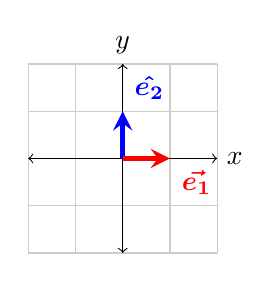
\begin{tikzpicture}[scale=0.6]
  \draw[thin,gray!40] (-2,-2) grid (2,2);
  \draw[<->] (-2,0)--(2,0) node[right]{$x$};
  \draw[<->] (0,-2)--(0,2) node[above]{$y$};
  \draw[line width=2pt,blue,-stealth](0,0)--(0,1) node[anchor=south west]{$\boldsymbol{\hat{e_2}}$};
  \draw[line width=2pt,red,-stealth](0,0)--(1,0) node[anchor=north west]{$\boldsymbol{\vec{e_1}}$};
\end{tikzpicture}
\end{center}
\begin{align*}
    && Span(\{\vec{e_1}, \vec{e_2}\}) &= \mathbb{R}^2 && \\
    && (x, y) &= x \cdot \vec{e_1} + y \cdot \vec{e_2} && \forall x, y \in \mathbb{R}
\end{align*}
\end{tcolorbox}
\theoremstyle{definition}
\begin{definition}{\textbf{Linearly dependent: }}
If $\vec{z} \in Span(X)$, $\vec{z}$ is \textbf{linearly dependent} on $X$.
\end{definition}
\theoremstyle{definition}
\begin{definition}{\textbf{Basis: }}
If $Span(X) = V$, $X$ forms a \textbf{basis} for $V$.
\end{definition}
\theoremstyle{definition}
\begin{definition}{\textbf{Linearly Independent: }}
$X$ is \textbf{linearly independent} if $\forall i, x_i$ is linearly independent of $X | \{x_i\}$. In other words, $x_i$ cannot be formed by linear combination of $X | \{x_i\}$.
\end{definition}


\section{Rank}
\theoremstyle{definition}
\begin{definition}{\textbf{Rank: }}
\textbf{rank}(X) is the size of the largest subset of X that are linearly independent.
\end{definition}
$$ A = \begin{bmatrix}- \vec{a_1}- \\ -\vec{a_2}- \\ -\vdots -\\ -\vec{a_n}- \end{bmatrix}_{nxd}$$
\begin{align*}
    rank(A) &= rank(\{ \vec{a_1}, \dots, \vec{a_n} \}) \\
            &\leq min (n, d)
\end{align*}
\begin{fact}
Row rank = Column rank
\end{fact}
\begin{definition}{\textbf{Full Rank: }}
matrix $A$ has \textbf{full rank} if $rank(A) = min(n,d)$.
\end{definition}

\section{Inverse}
\begin{definition}{\textbf{Full Rank: }}
matrix $A$ is \textbf{square} if number of rows is equal to number of columns.
\end{definition}

A square matrix $A$ may or may not have an inverse, but if the inverse, $A^{-1}$, exists, it is the unique matrix satisfying 
$$A^{-1}A = AA^{-1} = \underbrace{I}_{identity matrix} = \begin{bmatrix} 
                    1 &  & 0 \\
                     & \ddots & \\
                    0 &  & 1 
                    \end{bmatrix}$$

\begin{theorem}
Let A be a square matrix,
$$\text{A is invertible} \Longleftrightarrow \text{A has a full rank} $$
\end{theorem}

\section{Orthogonality}

\begin{definition}
Let $\vec{x}, \vec{y} \in \mathbb{R}^d$,
$$\langle \vec{x}, \vec{y} \rangle = 0 \equiv \text{$\vec{x}$ and $\vec{y}$ are \textbf{orthogonal}}$$
\end{definition}

\begin{definition}
Let $A$ be a matrix,
if every column $c_i$ of $A$ is a unit vector (normalized with $\norm{c_i} = 1$) and each column is orthogonal to other column vectors, $A$ is \textbf{orthonormal}.
\end{definition}

\begin{definition}
if every column $c_i$ of $A$ is a unit vector (normalized with $\norm{c_i} = 1$) and each column is orthogonal to other column vectors, $A$ is \textbf{orthonormal}.
\end{definition}

\begin{definition}
A square matrix $U \in \mathbb{R}^{nxn}$ whose rows and columns are orthonormal is called an \textbf{orthogonal matrix}.
\end{definition}

\begin{fact}
Let $U \in \mathbb{R}^{nxn}$ be an orthogonal matrix,
\begin{align}
    U^TU = I = UU^T\\
    U^{-1} = U^T
\end{align}
\end{fact}

\begin{lemma}
If $Q$ is orthonormal, then $\forall \vec{x} \in \mathbb{R}^n, \norm{Q\vec{x}}_2 = \norm{\vec{x}}_2$
\end{lemma}
\begin{proof}
\begin{align*}
    \norm{Q\vec{x}}_2^2 &= (Q\vec{x})^T(Q\vec{x}) \\                
    \norm{Q\vec{x}}_2^2 &= \vec{x}^T\underbrace{Q^TQ}_{I}\vec{x} \\
    \norm{Q\vec{x}}_2^2 &= \vec{x}^T\vec{x} \\
    \norm{Q\vec{x}}_2^2 &= \norm{\vec{x}}_2^2 \\
    \norm{Q\vec{x}}_2 &= \norm{\vec{x}}_2
\end{align*}
\end{proof}
\begin{lemma}
If $Q$ is orthonormal, then for any matrix $A$
$$\norm{QA} = \norm{A}$$
\end{lemma}
\begin{proof}
\begin{align*}
    && \norm{Q\vec{x}}_2 &= max_{\hat{x} \in \mathbb{R}^n, \norm{\hat{x}} = 1} \norm{Q\underbrace{(A\hat{x})}_{\text{also a vector}}}_2 && \\                
    &&                  &= max_{\hat{x} \in \mathbb{R}^n, \norm{\hat{x}} = 1} \norm{A\hat{x}}_2 && \text{(by Lemma 7.6)} \\
    && &= \norm{A} && \text{(by definition of Spectral norm)}
\end{align*}
\end{proof}

\section{Eigen Value \& Eigen Vector}

Let $A$ be $n\times n$ matrix then
\[
Ax = \lambda x
\]
We call $x$ is the "Eigen Vector" of $A$ with the corresponding "Eigen Value" $\lambda$. The intuition here is that $x$ maintains the direction when multiply by A, hence it only changes the length.
\\
It is possible that for eigen value, $\lambda$,
\begin{align*}
Ax &= \lambda x\\
Ay &= \lambda y\\
\text{then}\\
A(\alpha x+\beta y) &= \lambda (\alpha x + \beta y)
\end{align*}

\begin{definition}
 	Let $A, B$ be matrix, $A,B$ are similar if there exists an invertible matrix $P$ such that
 	\[
 		A=P^{-1}BP
 	\]
 	If $A$ and $B$ are similar, then they have the same eigen value
\end{definition}
\begin{proof}
	\begin{align*}
	A&=P^{-1}BP\\
	PA&=BP \quad(1)\\
	\text{Let } Ax &=\lambda x\\
	\pmb{P}Ax &= \lambda \pmb{P}x\\
	\pmb{BP}x &= \lambda Px\quad \text{from } (2)\\
	B\pmb{Px} &= \lambda \pmb{Px} \quad \blacksquare.
	\end{align*}
	Thus we have eigen vecgor $Px$ with corresponding eigenvalue $\lambda$
\end{proof}
\begin{definition}
	Matrix $A$ is diagonalizable if $A$ is similar to a diagonal matrix. Recall that a diagonal matrix is matrix where all $x_{ij}$ are 0 except when $i=j$.
\end{definition}
\begin{theorem}
	$A$ is diagonalizable if and only if $A$ has $n$ linearly independent Eigen vector
\end{theorem}
\begin{proof}[Proof (=>)]
	Suppose there exists matrix $D$ such that $D = P^{-1}AP$ then
	\begin{align*}
	D &= P^{-1}AP\\
	PD &= AP\\
	\left[
	\begin{matrix}
		\vline &\vline&\dots&\vline\\
		P_1 & P_2 & \dots& P_n\\
		\vline &\vline&\dots&\vline\\
		\vline &\vline&\dots&\vline\\
	\end{matrix}
	\right]
	\left[
	\begin{matrix}
	\delta_1 & &  & 0\\
	 & \delta_2& &	\\
	&  & \ddots &\\
	0 & & & \delta_n
	\end{matrix}
	\right]
	&= A\left[
	\begin{matrix}
	\vline &\vline&\dots&\vline\\
	P_1 & P_2 & \dots& P_n\\
	\vline &\vline&\dots&\vline\\
	\vline &\vline&\dots&\vline\\
	\end{matrix}
	\right]\\
	\left[
	\begin{matrix}
	\vline &\vline&\dots&\vline\\
	\delta_1 P_1 & \delta_2P_2 & \dots& \delta_nP_n\\
	\vline &\vline&\dots&\vline\\
	\end{matrix}
	\right] &= \left[
	\begin{matrix}
	\vline &\vline&\dots&\vline\\
	AP_1 & AP_2 & \dots& AP_n\\
	\vline &\vline&\dots&\vline\\
	\end{matrix}
	\right]
	\end{align*}
	Since $P$ is invertible then $P$ has full rank and therefore $P$ is linearly independent
\end{proof}

\begin{proof}[Proof (<=)]
	Do the [=>] part in reverse order
\end{proof}
\begin{definition}
	$A$ is orthogonally diagonalizable (OD) if there exists $P$ which is orthogonal such that $P^{-1}AP$ is diagonal.
\end{definition}
\begin{claim}
	If $A$ is OD then $A=PDP^T$
	\begin{align*}
	A &= PDP^T\\
	&=\sum{i=1}^n d_{ii}P_iP_i^T
	\end{align*}
\end{claim}
\begin{theorem}[Spectral Theorem for Real Matrices]
	$ $\\
	Let $A$ be a real symmetric matrix, then
	\begin{enumerate}
		\item The eigen value $\lambda_i$ are reals and the eigen vectors are real
		\item $A$ is OD so \\
		\begin{align*}
		A &= \left[
		\begin{matrix}
		\vline &\dots&\vline\\
		V_1 & \dots& V_n\\
		\vline &\dots&\vline\\
		\end{matrix}
		\right]
		\left[
		\begin{matrix}
		\lambda_1 & &  & 0\\
		& \lambda_2& &	\\
		&  & \ddots &\\
		0 & & & \lambda_n
		\end{matrix}
		\right]
		\left[
		\begin{matrix}
		- &V_1&-\\
		&\vdots& \\
		-&V_n&-
		\end{matrix}
		\right]\\
		&= VDV^T\\
		&=\sum_{i=1}^n\lambda_n V_iV_i^T
		\end{align*}
	\end{enumerate}
\end{theorem}

\begin{theorem}[The Fundamental Theorem of Symmetric Matrices]
	$ $ \newline A real matrix $A$ is OD $\iff$ $A$ is symmetric.
\end{theorem}
%Finally, if you have citations, see the commented-out stuff in the \LaTeX~here.

%\

%My farourive Optimization books are \cite{bertsimas1997introduction} \cite{boyd2004convex} \cite{wolsey2014integer}. You should add bibliographical notes in the \textbf{BibTex}: \textit{mybib.bib} file. Its good to grab these notes from Google scholar citations.

%%%%%%%%%% If you don't have citations then comment the lines below:

%\bibliographystyle{abbrv}           % if you need a bibliography
%\bibliography{mybib}                % assuming yours is named mybib.bib


%%%%%%%%%%% end of doc
\end{document}

